\documentclass[a4paper]{arrowhead}

\usepackage[yyyymmdd]{datetime}
\usepackage{etoolbox}
\usepackage[utf8]{inputenc}
\usepackage{multirow}
\usepackage{hyperref}

\renewcommand{\dateseparator}{-}

\setlength{\parskip}{1em}

%% Special references
\newcommand{\fref}[1]{{\textcolor{ArrowheadBlue}{\hyperref[sec:functions:#1]{#1}}}}
\newcommand{\mref}[1]{{\textcolor{ArrowheadPurple}{\hyperref[sec:model:#1]{#1}}}}
\newcommand{\pdef}[1]{{\textcolor{ArrowheadGrey}{#1\label{sec:model:primitives:#1}\label{sec:model:primitives:#1s}\label{sec:model:primitives:#1es}}}}
\newcommand{\pref}[1]{{\textcolor{ArrowheadGrey}{\hyperref[sec:model:primitives:#1]{#1}}}}

\newrobustcmd\fsubsection[3]{
  \addtocounter{subsection}{1}
  \addcontentsline{toc}{subsection}{\protect\numberline{\thesubsection}operation \textcolor{ArrowheadBlue}{#1}}
  \renewcommand*{\do}[1]{\rref{##1},\ }
  \subsection*{
    \thesubsection\quad
    operation
    \textcolor{ArrowheadBlue}{#1}
    (\notblank{#2}{\mref{#2}}{})
    \notblank{#3}{: \mref{#3}}{}
  }
  \label{sec:functions:#1}
}
\newrobustcmd\msubsection[2]{
  \addtocounter{subsection}{1}
  \addcontentsline{toc}{subsection}{\protect\numberline{\thesubsection}#1 \textcolor{ArrowheadPurple}{#2}}
  \subsection*{\thesubsection\quad#1 \textcolor{ArrowheadPurple}{#2}}
  \label{sec:model:#2} \label{sec:model:#2s} \label{sec:model:#2es}
}

\begin{document}

%% Arrowhead Document Properties
\ArrowheadTitle{TranslationManager Support System}
\ArrowheadType{System Description}
\ArrowheadTypeShort{SysD}
\ArrowheadVersion{5.1.0}
\ArrowheadDate{\today}
\ArrowheadAuthor{Rajmund Bocsi}
\ArrowheadStatus{DRAFT}
\ArrowheadContact{rbocsi@aitia.ai}
\ArrowheadFooter{\href{www.arrowhead.eu}{www.arrowhead.eu}}
\ArrowheadSetup
%%

%% Front Page
\begin{center}
  \vspace*{1cm}
  \huge{\arrowtitle}

  \vspace*{0.2cm}
  \LARGE{\arrowtype}
  \vspace*{1cm}

  %\Large{Service ID: \textit{"\arrowid"}}
  \vspace*{\fill}

  % Front Page Image
  %\includegraphics{figures/TODO}

  \vspace*{1cm}
  \vspace*{\fill}

  % Front Page Abstract
  \begin{abstract}
    This document provides system description for the \textbf{TranslationManager Support system}.
  \end{abstract}

  \vspace*{1cm}

 \end{center}

\newpage
%%

%% Table of Contents
\tableofcontents
\newpage
%%

\section{Overview}
\label{sec:overview}
\color{black}
This document describes the TranslationManager Support system, which exists to help the communication between a consumer and a provider if there is no common interface between them and/or are using different data models.  The TranslationManager achieves this goal by building a translation bridge using various translator systems (application systems) as building blocks. An other example of such help is the ability to determine the possibility to build such bridge with the currently available translators.

The rest of this document is organized as follows.
In Section \ref{sec:prior_art}, we reference major prior art capabilities
of the system.
In Section \ref{sec:use}, we describe the intended usage of the system.
In Section \ref{sec:properties}, we describe fundamental properties
provided by the system.
In Section \ref{sec:delimitations}, we describe delimitations of capabilities
of the system.
In Section \ref{sec:services}, we describe the abstract services produced by the system.
In Section \ref{sec:security}, we describe the security capabilities
of the system.

\subsection{Significant Prior Art}
\label{sec:prior_art}

The strong development on cloud technology and various requirements for digitization and automation has led to the concept of Local Clouds (LC).

One of the main issue when realizing such Local Cloud is that multiple applications have to cooperate with each other. Some of these applications are legacy systems with their own interfaces and data models and unable to use new standards. The lack of interoperability can be a real problem, and one solution for this issue is to modify existing applications. A better solution to provide some proxy entities that can achieve interoperability by translating data during the communication.

The TranslationManager Support system can build such proxies by utilizing various translator components (application systems that can translate between interfaces or between different data models).

The previous versions of the Arrowhead Framework (4.6.x) have a system (translator) that offers similar functionality, but it want to contain all translation related logic in one system. It provides very limited options for translation and every new option would require additional coding in the translator Support system.

In case of the TranslationManager system, its usefulness can be increased by deploying new interface and/or data model translators into the Local Cloud, and the Support system can use them without any additional requirement.

\subsection{How This System Is Meant to Be Used}
\label{sec:use}

TranslationManager is a Support system of Eclipse Arrowhead Local Cloud and is responsible for building communication bridges between application systems that can't communicate each other directly. 

A service orchestration Core system can use the TranslationManager's functionality to offer a service instance for the consumer even there is no exact match for the interface requirements. Figure \ref{fig:translation_process} describes this use case.

Additionally, a consumer can consume the TranslationManager's translationBridge service to determine which service instance candidates can be use via translation bridge. If such service instance exists, the consumer can ask the TranslationManager to build the translation bridge.

\begin{figure}[ht!]
  \centering
  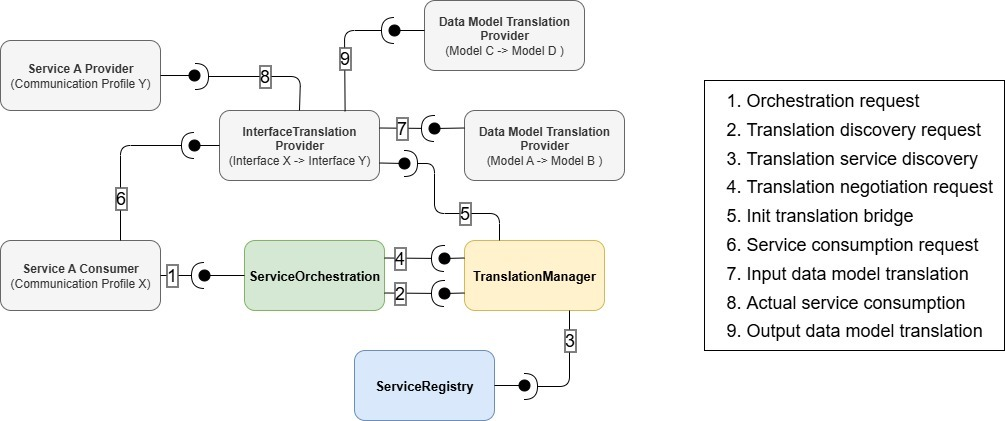
\includegraphics[width=\textwidth]{figures/TranslatorManagerv5.jpg}
  \caption{Translation process with a service orchestration system}
  \label{fig:translation_process}
\end{figure}

\subsection{System functionalities and properties}
\label{sec:properties}

\subsubsection {Functional properties of the system}
TranslationManager solves the following needs to fulfill the requirements of handling translation bridges.

\begin{itemize}
    \item Enables to consumers to discover translation bridge building possibilities for a service operation.
    \item Enables to consumers to build a translation bridge for a service operation.
    \item Enables to consumers to abort previously built translation bridges.
    \item Enables to Core/Support systems to discover translation bridge building possibilities for a service operation in the name of a consumer.
    \item Enables to Core/Support systems to build a translation bridge for a service operation in the name of a consumer.
    \item Enables to Core/Support systems to abort existing translation bridges in bulk.
    \item Enables to Core/Support systems to query translation bridge (currently active and old ones) details using various filters.
    \item Enables to interface translators to send reports about their translation bridges.
\end{itemize}

\subsubsection {Non functional properties of the system}

\begin{itemize}
    \item If an Authentication system is present in the Local Cloud, the TranslationManager will use its service(s) to verify a requester system before responding to its request.
    \item If X.509 authentication policy is used instead of a dedicated Authentication system, the TranslationManager will verify the provided certificate before any response.
    \item If the ConsumerAuthorization system is present in the Local Cloud, the TranslationManager may use its service(s) to check the permissions about target providers' and the used translators' services.
    \item If the Blacklist system is present in the Local Cloud, the TranslationManager may use its service(s) to check requesters, consumers and translators.
    \item If a Configuration system is present in the Local Cloud, the TranslationManager may use its service(s) to load custom configuration related to the translators.
\end{itemize}
 

\subsubsection {Data stored by the system}
In order to achieve the mentioned functionalities, TranslationManager is capable to store the following information set:

\begin{itemize}
    \item \textbf{Bridge discovery}: The results of a discovery operation. Every entity describes a service instance whose operation can be accessed via a translation bridge. Can be removed after actual bridge creation.
    \item \textbf{Bridge details}: Information about a translation bridge.
\end{itemize}

\subsection{Important Delimitations}
\label{sec:delimitations}

\begin{itemize}
    \item If the Local Cloud does not contain an Authentication system or does not using X.509 certificates, there is no way for the TranslationManager to verify the requester system. In that case, the TranslationManager will consider the authentication data that comes from the requester as valid.
    \item TranslationManager can't work alone. For every translation bridge it needs an appropriate 
    interface translator and optionally one or two data model translators. These translators are ordinary providers registered in the ServiceRegistry.
\end{itemize}

\newpage

\section{Services produced}
\label{sec:services}

\phantomsection
\msubsection{service}{translationBridge}
The purpose of this service is to find providers whose service operation is accessible by the requester via a translation bridge using the currently available translators and to build/abort such bridges. This service is offered for Application systems (consumers). 

\msubsection{service}{translationReport}
The purpose of this service is to provide a tool to send events about translation bridges. This service is offered for interface translator systems.

\msubsection{service}{translationBridgeManagement}
The purpose of this service is to find providers whose service operation is accessible by a specified consumer via a translation bridge using the currently available translators and to build such bridges. It also offers bulk abortion and query functionalities. This service is offered for Core/Support systems.

\msubsection{service}{monitor}
Recommended service. Its purpose is to give information about the provider system. The service is offered for both application and Core/Support systems.

\newpage

\section{Security}
\label{sec:security}

For authentication, the TranslationManager can utilize an other core system, the Authentication system's service to verify the identities of the requester systems. If no Authentication system is deployed into the Local Cloud, the TranslationManager can accept X.509 certificates for identification. If none of these are available, the TranslationManager trusts the requester system's self-provided identity.

For authorization, \textit{translationBridge} is available for everyone who can get access information via service orchestration (or directly from the ServiceRegistry, if direct lookup is allowed in the Local Cloud). The \textit{translationBridgeManagement} service is available those who has the appropriate permissions. The \textit{translationReport} is only available for interface translators and every interface translator can only report about their own translation bridges.

The implementation of the TranslationManager can decide about the encryption of the connection between the TranslationManager and other systems. 

\newpage

\bibliographystyle{IEEEtran}
\bibliography{bibliography}

\newpage

\section{Revision History}
\subsection{Amendments}

\noindent\begin{tabularx}{\textwidth}{| p{1cm} | p{3cm} | p{2cm} | X | p{4cm} |} \hline
\rowcolor{gray!33} No. & Date & Version & Subject of Amendments & Author \\ \hline

1 & YYYY-MM-DD & \arrowversion & & Xxx Yyy \\ \hline
\end{tabularx}

\subsection{Quality Assurance}

\noindent\begin{tabularx}{\textwidth}{| p{1cm} | p{3cm} | p{2cm} | X |} \hline
\rowcolor{gray!33} No. & Date & Version & Approved by \\ \hline

1 & YYYY-MM-DD & \arrowversion  &  \\ \hline

\end{tabularx}

\end{document}